\begin{figure}[!t]
\centering
\includegraphics[width=3in]{phi-level}
\caption{Scenario I}
\label{fig:model:phi-level}
\end{figure}

\section{Implementation Progression}
The fundamental concepts demonstrated in our prototypes are those related to usage management in multi-level-security cross-domain environments. We provide prototypes that clearly demonstrate the research concepts that are being investigated. Below are some very high-level scenarios we have built. We have purposefully abstracted out specifics such as the type of the domain (i.e. NIPRnet, SIPRnet, etc.), as well as implementation-specific issues, such as whether or not some functionality is implemented as a virtual machine, the type of data repository, and so on. The focus in these scenarios is demonstrating the fundamental design concepts embodied in the scenarios.

\subsection{Scenario I}
In this scenario the cross-domain solution (CDSO is a $\phi$ guard. A user in Domain B makes an information request, and this leads to document request. The appropriate document is retrieved, and passes through the guard if it passes all of the filters associated with the guard; otherwise the document is dropped for reliable human review.

The set of filters that could be developed and deployed within the guard are unlimited.  Developers could easily create a filter that inspects and possibly redacts the sections within the document, rather than passing or not passing the entire document through the guard.  Indeed, if we assume even very limited processing capabilities within the guard, that is, turing completeness, then this guard can be made as powerful as any solution we can derive for implementing a CDS. Thus the computational power of the guard is not the issue. The real issues are the benefits that can be gained by distributing the capabilities intelligently within the networked environment.

Note that in Scenario I, once content is delivered to Domain B, it is no longer managed.

\subsection{Scenario II --- Policy-Content Separation}
In this scenario the CDS is an $\alpha$ guard. The fundamental design concept this scenario demonstrates is the policy-content separation principle. That is, content and policy should not be intertwined within one document.  This principle is similar to the one behind the form-content separation principle. This is the principle that led to CSS files containing form, and HTML documents containing pure content-related elements. Similarly, the behavior-content principle, embodied in unobtrusive JavaScript, has recently been recognized as an important design principle. Thus, in this scenario we are extending these ideas to what we are calling the policy-content separation principle.

\begin{figure}[!t]
\centering
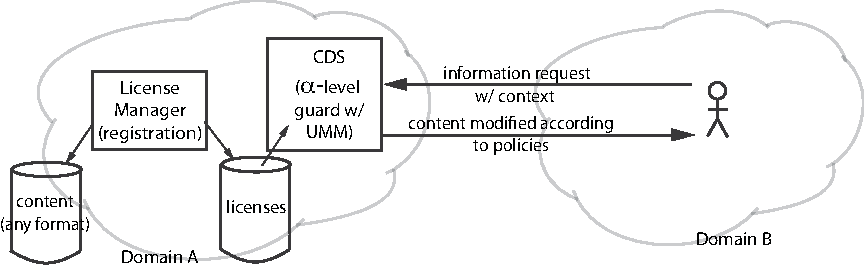
\includegraphics[width=3in]{alpha-level-1}
\caption{Scenario II}
\label{fig:model:alpha-level-1}
\end{figure}

For the purpose of this scenario, we demonstrate more sophisticated cross-domain transfer capabilities.  We create XML documents, and then apply policies to the various sections of these documents, and then show how pieces of a document can be passed through the CDS, while other pieces are filtered out. In addition, we change a policy in one place (within a license), and demonstrate how this one policy change can impact how hundreds of documents are now managed.  This way, a single license can be applied to a potentially unlimited number of resources.

Here, we have essentially built an access control solution, albeit more sophisticated than the previous one. In this scenario, the policies are no longer centralized within the guard, rather they are separated.  Also, note that although we show a content repository only, we can easily extend the polices in our usage management framework to services.

\subsection{scenario III --- End-to-End Arguments}
In this scenario the CDS is also an $\alpha$ guard; however, usage management is now fully implemented within Domain B.

This architectural change now fully enables usage management across the two domains, while at the same time pushing usage management functionality closer to the end points. In addition, the usage management functionalities are also more distributed, leading to the creation of additional roles within each domain. Specifically, in Scenario 1, the policy is wrapped up inside the guard, and only someone that has the authority to modify the guard can modify the policy. In this scenario, the policy has been removed from the CDS, and therefore someone with authority inside of the domain can set the policy. This, presumably would require less authority that modifying a CDS. The CDS's job now is simply to interpret and enforce policy --- policy is no longer stored in the CDS itself. Furthermore, in this scenario we have moved beyond access control, and are now able to implement usage management use cases, e.g., we can retract content from Domain B according to certain circumstances. This is a very important use case to demonstrate related to managing content within coalition partner domains.

An important level of detail we can bring into this prototype scenario is the notion that the license and context are expressed according to ontologies that are domain specific. This leads to a very interesting and difficult research problem --- specificall how one domain recognizes a license that has been created according to an ontology in a different domain. One way to solve this problem is to assume that ontologies are organized according to inheritance hierarchy.

In this figure it may be the case that both domain A and B do not want the other to know the actual elements that are included in their ontologies; however, both of them are based upon ontologies that are publically available, or at least available across the domains.

In the scenario above, let us assume that an ontology is known to both domains, and Domain B has informed Domain A that it can receive licenses that are built according to that ontology. Thus, the usage management mechanism (UMM) within Domain A must first determine if it can create a license that satisfies the required polices of the requested content object. If it can, then it can use the more general ontology, create a license, and send it to Domain B. The UMM within Domain B can now appropriately manage, according to the original policies, the content it has received within its own domain.

The separation of ontology from the license manager in this case also allows for the development of stand-alone content generation and license checking capabilities.

\begin{figure}[!t]
\centering
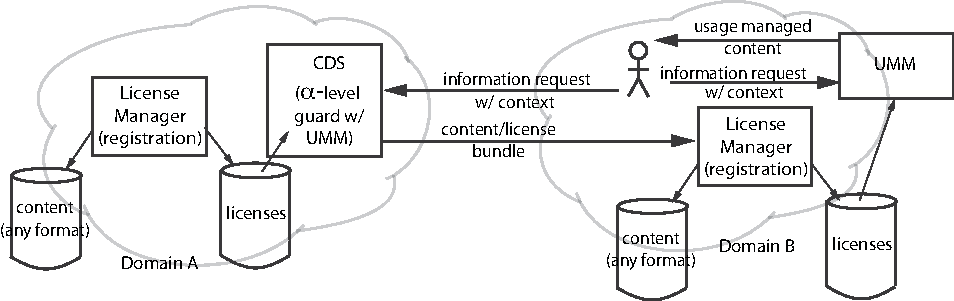
\includegraphics[width=3in]{alpha-level-2}
\caption{Scenario III}
\label{fig:model:alpha-level-2}
\end{figure}